\subsection{Pipeline stages}

In order to build a pipeline, many things have to be taken into account. The slowest pipeline stage determines the maximum frequency at which the processor runs. The instructions have to be passed down the pipeline, and the decoding can be done as the instruction is being executed. The MIPS pipeline is divided into five non interlocked pipeline stages as shown in Figure \ref{pipelinestages}. Most of the wires in the picture are buses which means a bunch of wires which hold and transfer a given value or instruction.

\begin{figure}[!h]
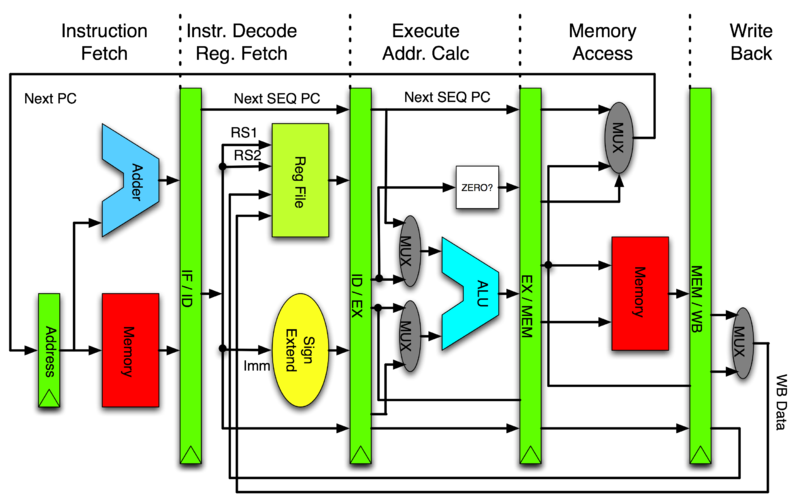
\includegraphics[width=0.45\textwidth]{Images/pipemips.png}
\caption{MIPS pipeline stages}
\label{pipelinestages}
\end{figure}

\subsubsection{IF: Instruction fetch}

In this stage the 32-bit instruction is being fetched from the memory using the address from the program counter. This instruction is stored in the IF/ID pipeline register. The address is then incremented by four since there are four bytes per word. The processor cannot at this stage know what type of instruction is fetched, so it must prepare for any instruction, and passing all potentially needed information to the next stage in the pipeline. 

A number of control signals are fed back to this stage from later stages, in order to handle jumps and branches, that require the program counter to be altered.

\subsubsection{ID: Instruction decode}

In this stage, the contents of two registers are fetched, based on the instruction word propagated from the IF/ID pipeline register. The two 32 bit values are then stored in the ID/EX registers. At this point the type of instruction is still not determined, so the registers are read, regardless of whether they are needed or not. Because this stage is executed regardless of the instruction no control signals are needed, but the control signals for the subsequent stages are extracted here, and propagated along in the pipeline registers.

\subsubsection{EX: Execute stage}

In this stage different things can happen,  on of the values of the read register is passed on to the EX/MEM pipeline register to be used in case of a memory operation. The two register values can be processed by an arithmetic operation in the ALU and passed on to the EX/MEM register. The instruction can be a branch or a jump instruction and thus a new PC can be calculated. The value of the new PC is stored in the EX/MEM pipeline registers.

In this stage, a number of control signals are needed. The control signal for this stage contains three values that control different multiplexers: an ALU control, a register control and a PC control. The MUX for the PC is not directly controlled, but the signal value is stored in the EX/MEM pipeline register.  

\subsubsection{MEM: Memory stage}

The MEM stage reads the EX/MEM pipeline registers and reads from, or writes to the main memory. In case of a read, the data is passed to the MEM/WB pipeline register. This is the stage where the jump functions take effect and the PC is updated. The thing to notice is jump functions only take four stages in the MIPS pipeline compared to all other functions that takes five. If the jump function is a reality the pipeline, given that the branch prediction was wrong, has to be flushed. Two control signals are needed in this stage, one to control the memory read or write and the second is for branching.

\subsubsection{WB: Write back}

The write back stage reads the MEM/WB pipeline register and stores the value back into the registers. If the instruction was a memory write, a jump function or a NOP nothing happens in this stage. This stage is the final stage in the MIPS pipeline, and thus the instruction is completed after this step. Some of the more advanced arithmetic operations (multiply, divide etc.) are exceptions to this rule, as they take multiple clock cycles to complete. However, they are performed in the backgroung, and the result will be written to reserved registers, when they are ready. It is therefore up to the compiler / programmer, to make sure that the data is ready, before attempting to read the result. If this \textit{background} approach is not taken, the frequency of the processor has to be lowered to fit the complex instructions, which would severely increase the latency and thus lower the throughput of the processor. 

